\documentclass[12pt,a4paper,openany]{ctexrep}

% 页面设置
\usepackage[top=2.5cm, bottom=2.5cm, left=3cm, right=3cm]{geometry}
\usepackage{graphicx}
\usepackage{booktabs}
\usepackage{longtable}
\usepackage{tabularx}
\usepackage{listings}
\usepackage{xcolor}
\usepackage{hyperref}
\usepackage{enumitem}
\usepackage{setspace}
\usepackage{caption}

% 行距
\onehalfspacing

% 首行缩进
\setlength{\parindent}{2em}

% 超链接样式
\hypersetup{
  colorlinks=true,
  linkcolor=blue!70!black,
  urlcolor=blue!70!black,
  bookmarksnumbered=true,
  pdfauthor={陈林峰},
  pdftitle={iGEM Dry Team 项目实施计划方案}
}

% 代码样式
\lstset{
  basicstyle=\small\ttfamily,
  keywordstyle=\color{blue!70!black},
  stringstyle=\color{red!60!black},
  commentstyle=\color{green!50!black},
  backgroundcolor=\color{gray!5},
  frame=single,
  rulecolor=\color{gray!30},
  breaklines=true,
  showstringspaces=false,
  tabsize=2,
  columns=flexible
}

% 图片搜索路径
\graphicspath{{../figure/}{../../hardware/figure/}}

% 标题信息
\title{\textbf{iGEM Dry Team 项目实施计划方案} \\ \large （完善版）}
\author{陈林峰}
\date{2026年4月22日}

\begin{document}

\maketitle
\tableofcontents
\newpage

%=============================================================================
\chapter{项目定位与总目标}
%=============================================================================

项目目标是构建一套无人机投放工程菌检测节点的闭环系统，用于实时监测与预警水体藻毒素风险。

\section{当前真实状态（2026-04-22）}

\begin{table}[htbp]
\centering
\caption{各模块当前状态}
\begin{tabularx}{\textwidth}{l l X}
\toprule
\textbf{模块} & \textbf{状态} & \textbf{关键进展} \\
\midrule
数学建模 & 已完成全流程 & 3 数据集 (HABs/Lake Erie/SF Estuary) 清洗、XGBoost+LightGBM 集成训练、SHAP 解释，Lake Erie 分类 AUC=0.943 \\
检测装置 & 面包板 Demo & 3D 结构设计 + 实物验证完成，PCB 版本待开发 \\
Web 平台 & Demo 展示 & 总览/设备配对/数据分析/地图页已搭建，实时数据流待接入 \\
无人机系统 & 未开发 & 部件采购完成，闭环中断点在"任务执行与投放"环节 \\
\bottomrule
\end{tabularx}
\end{table}

\section{现实化阶段目标}

\begin{enumerate}[label=M\arabic*（)]
\item 可演示：三个 Demo 可稳定复现，统一输入输出协议。
\item 可联调：检测端、模型端、网页端打通，支持模拟任务闭环。
\item 可外场：无人机完成可控试飞与投放，形成真实外场最小闭环。
\item 可答辩：闭环可重复运行，具备对照实验和完整评审证据。
\end{enumerate}

系统核心闭环如下：
\begin{enumerate}
\item 预测模型输出时空风险与不确定性。
\item 调度系统生成飞行与投放任务。
\item 无人机执行任务并投放检测节点。
\item 节点回传实测数据与设备状态。
\item 模型增量更新并重新决策下一轮任务。
\end{enumerate}

最终交付物：
\begin{enumerate}
\item 可运行的预测与调度引擎。
\item 可执行的无人机投放与检测链路。
\item 可展示的 Web 态势大屏与复盘系统。
\item 可答辩的 iGEM 评审证据包。
\end{enumerate}

%=============================================================================
\chapter{计算生物学模块（辅助 Wet 组）}
%=============================================================================

\section{目标}

用计算生物学手段降低 Wet 实验试错成本，提升工程菌构建效率。

\section{输入}

\begin{enumerate}
\item 藻毒素相关靶蛋白与候选受体序列。
\item 文献中已报道的结合位点与突变信息。
\item Wet 组实验反馈结果。
\end{enumerate}

\section{输出}

\begin{enumerate}
\item 候选结合位点排序清单。
\item 候选突变策略建议。
\item 每轮建议的证据说明与风险标注。
\end{enumerate}

\section{关键里程碑}

\begin{enumerate}
\item 完成毒素-受体候选库整理。
\item 完成一轮结构预测与对接筛选。
\item 输出可供 Wet 组直接测试的首批候选位点。
\end{enumerate}

\section{验收标准}

\begin{enumerate}
\item Wet 组可依据清单直接开展实验，不需要二次解释。
\item 每个候选位点都附带来源、评分与不确定性说明。
\end{enumerate}

%=============================================================================
\chapter{数学建模模块}
%=============================================================================

\section{子模块 A：藻毒素浓度预测}

\subsection{目标}

输出可解释、可部署的浓度预测与风险等级。

\subsection{输入}

\begin{enumerate}
\item 历史水质、气象、毒素数据。
\item 实时节点回传数据。
\item 外部天气预报数据。
\end{enumerate}

\subsection{输出}

\begin{enumerate}
\item 未来 24--72 小时风险热力图。
\item 红黄蓝分级预警结果。
\item 预测不确定性评分。
\end{enumerate}

\subsection{关键里程碑}

\begin{enumerate}
\item 统一特征工程与数据字典。\hfill\textcolor{green!60!black}{\textbf{已完成}}
\item 建立 XGBoost、LightGBM、Ensemble 基线对比。\hfill\textcolor{green!60!black}{\textbf{已完成}}
\item 增加 SHAP 解释与不确定性输出。\hfill\textcolor{green!60!black}{\textbf{已完成}}
\item 从 Demo 脚本升级为可重复运行的训练与推理流水线。\hfill\textcolor{green!60!black}{\textbf{已完成}}
\item 接入实时节点回传数据，实现在线推理。
\item 实现增量更新与模型版本管理。
\end{enumerate}

\subsection{当前进展}

已完成三个数据集的全流程建模（数据清洗 $\rightarrow$ 特征工程 $\rightarrow$ 模型训练 $\rightarrow$ 评估 $\rightarrow$ SHAP 解释）。

\subsubsection*{数据集规模}

\begin{table}[htbp]
\centering
\caption{建模数据集规模}
\begin{tabular}{llrr}
\toprule
\textbf{数据集} & \textbf{来源} & \textbf{样本数} & \textbf{特征维度} \\
\midrule
HABs Training & EPA NLA 全国湖泊调查 & 3,663 条 & 45 维 \\
Lake Erie & 伊利湖长期监测 & 2,659 条 & 23 维 \\
SF Estuary & 旧金山河口监测 & 437 条 & 25 维 \\
\bottomrule
\end{tabular}
\end{table}

\subsubsection*{核心性能指标（Ensemble 测试集）}

\begin{table}[htbp]
\centering
\caption{模型核心性能指标}
\begin{tabular}{lccc}
\toprule
\textbf{指标} & \textbf{HABs Training} & \textbf{Lake Erie} & \textbf{SF Estuary} \\
\midrule
分类 ROC-AUC & 0.847 & \textbf{0.943} & 0.811 \\
分类 F1 & 0.674 & \textbf{0.894} & 0.615 \\
回归 R$^{2}$ & 0.319 & \textbf{0.742} & 0.329 \\
回归 RMSE ($\mu$g/L) & 4.83 & 1.40 & 0.43 \\
\bottomrule
\end{tabular}
\end{table}

\textbf{SHAP 关键驱动因子：}叶绿素 a、总氮 (NTL)、水温、月份（季节性）在三个数据集中均为 Top 驱动因子。

详细评估报告见 \texttt{model/reports/dataset\_evaluation\_report.md}。

\subsection{待完成事项}

\begin{enumerate}
\item 接入节点实时数据流，替代历史数据推理。
\item 构建在线推理 API，支持 Web 平台调用。
\item 增加预测区间输出（不确定性量化）。
\item 按时间序列划分验证，替代随机划分。
\end{enumerate}

\subsection{当前模型输出示意}

毒素浓度风险热力图：

\begin{figure}[htbp]
\centering
\includegraphics[width=0.85\textwidth]{../figure/毒素浓度热力图.webp}
\caption{毒素浓度风险热力图}
\label{fig:heatmap}
\end{figure}

\section{子模块 B：空气动力学与扩散模型}

\subsection{目标}

实现投放命中修正与水体扩散评估。

\subsection{当前状态}

仅处于方案设计阶段，尚未形成可验证原型。

\subsection{输入}

\begin{enumerate}
\item 无人机飞行参数与载荷参数。
\item 风速风向与高度信息。
\item 水体流速与边界条件。
\end{enumerate}

\subsection{输出}

\begin{enumerate}
\item 投放风偏修正参数。
\item 检测节点覆盖半径评估。
\item 扩散趋势模拟结果。
\end{enumerate}

\subsection{验收标准}

\begin{enumerate}
\item 实测投放偏差显著低于无修正策略。
\item 扩散模拟与实测趋势方向一致。
\end{enumerate}

%=============================================================================
\chapter{硬件模块}
%=============================================================================

\section{ESP32 检测节点}

\subsection{目标}

实现低功耗、稳定、可回传的数据采集终端。

\subsection{当前进度}

已完成面包板 Demo 验证。当前 Demo 证据图如下：

检测装置三维结构设计图 1：

\begin{figure}[htbp]
\centering
\includegraphics[width=0.7\textwidth]{../../hardware/figure/3D模型1.webp}
\caption{检测装置三维结构设计图 1}
\label{fig:3d1}
\end{figure}

检测装置三维结构设计图 2：

\begin{figure}[htbp]
\centering
\includegraphics[width=0.7\textwidth]{../../hardware/figure/3D模型2.webp}
\caption{检测装置三维结构设计图 2}
\label{fig:3d2}
\end{figure}

检测装置实物 Demo 图：

\begin{figure}[htbp]
\centering
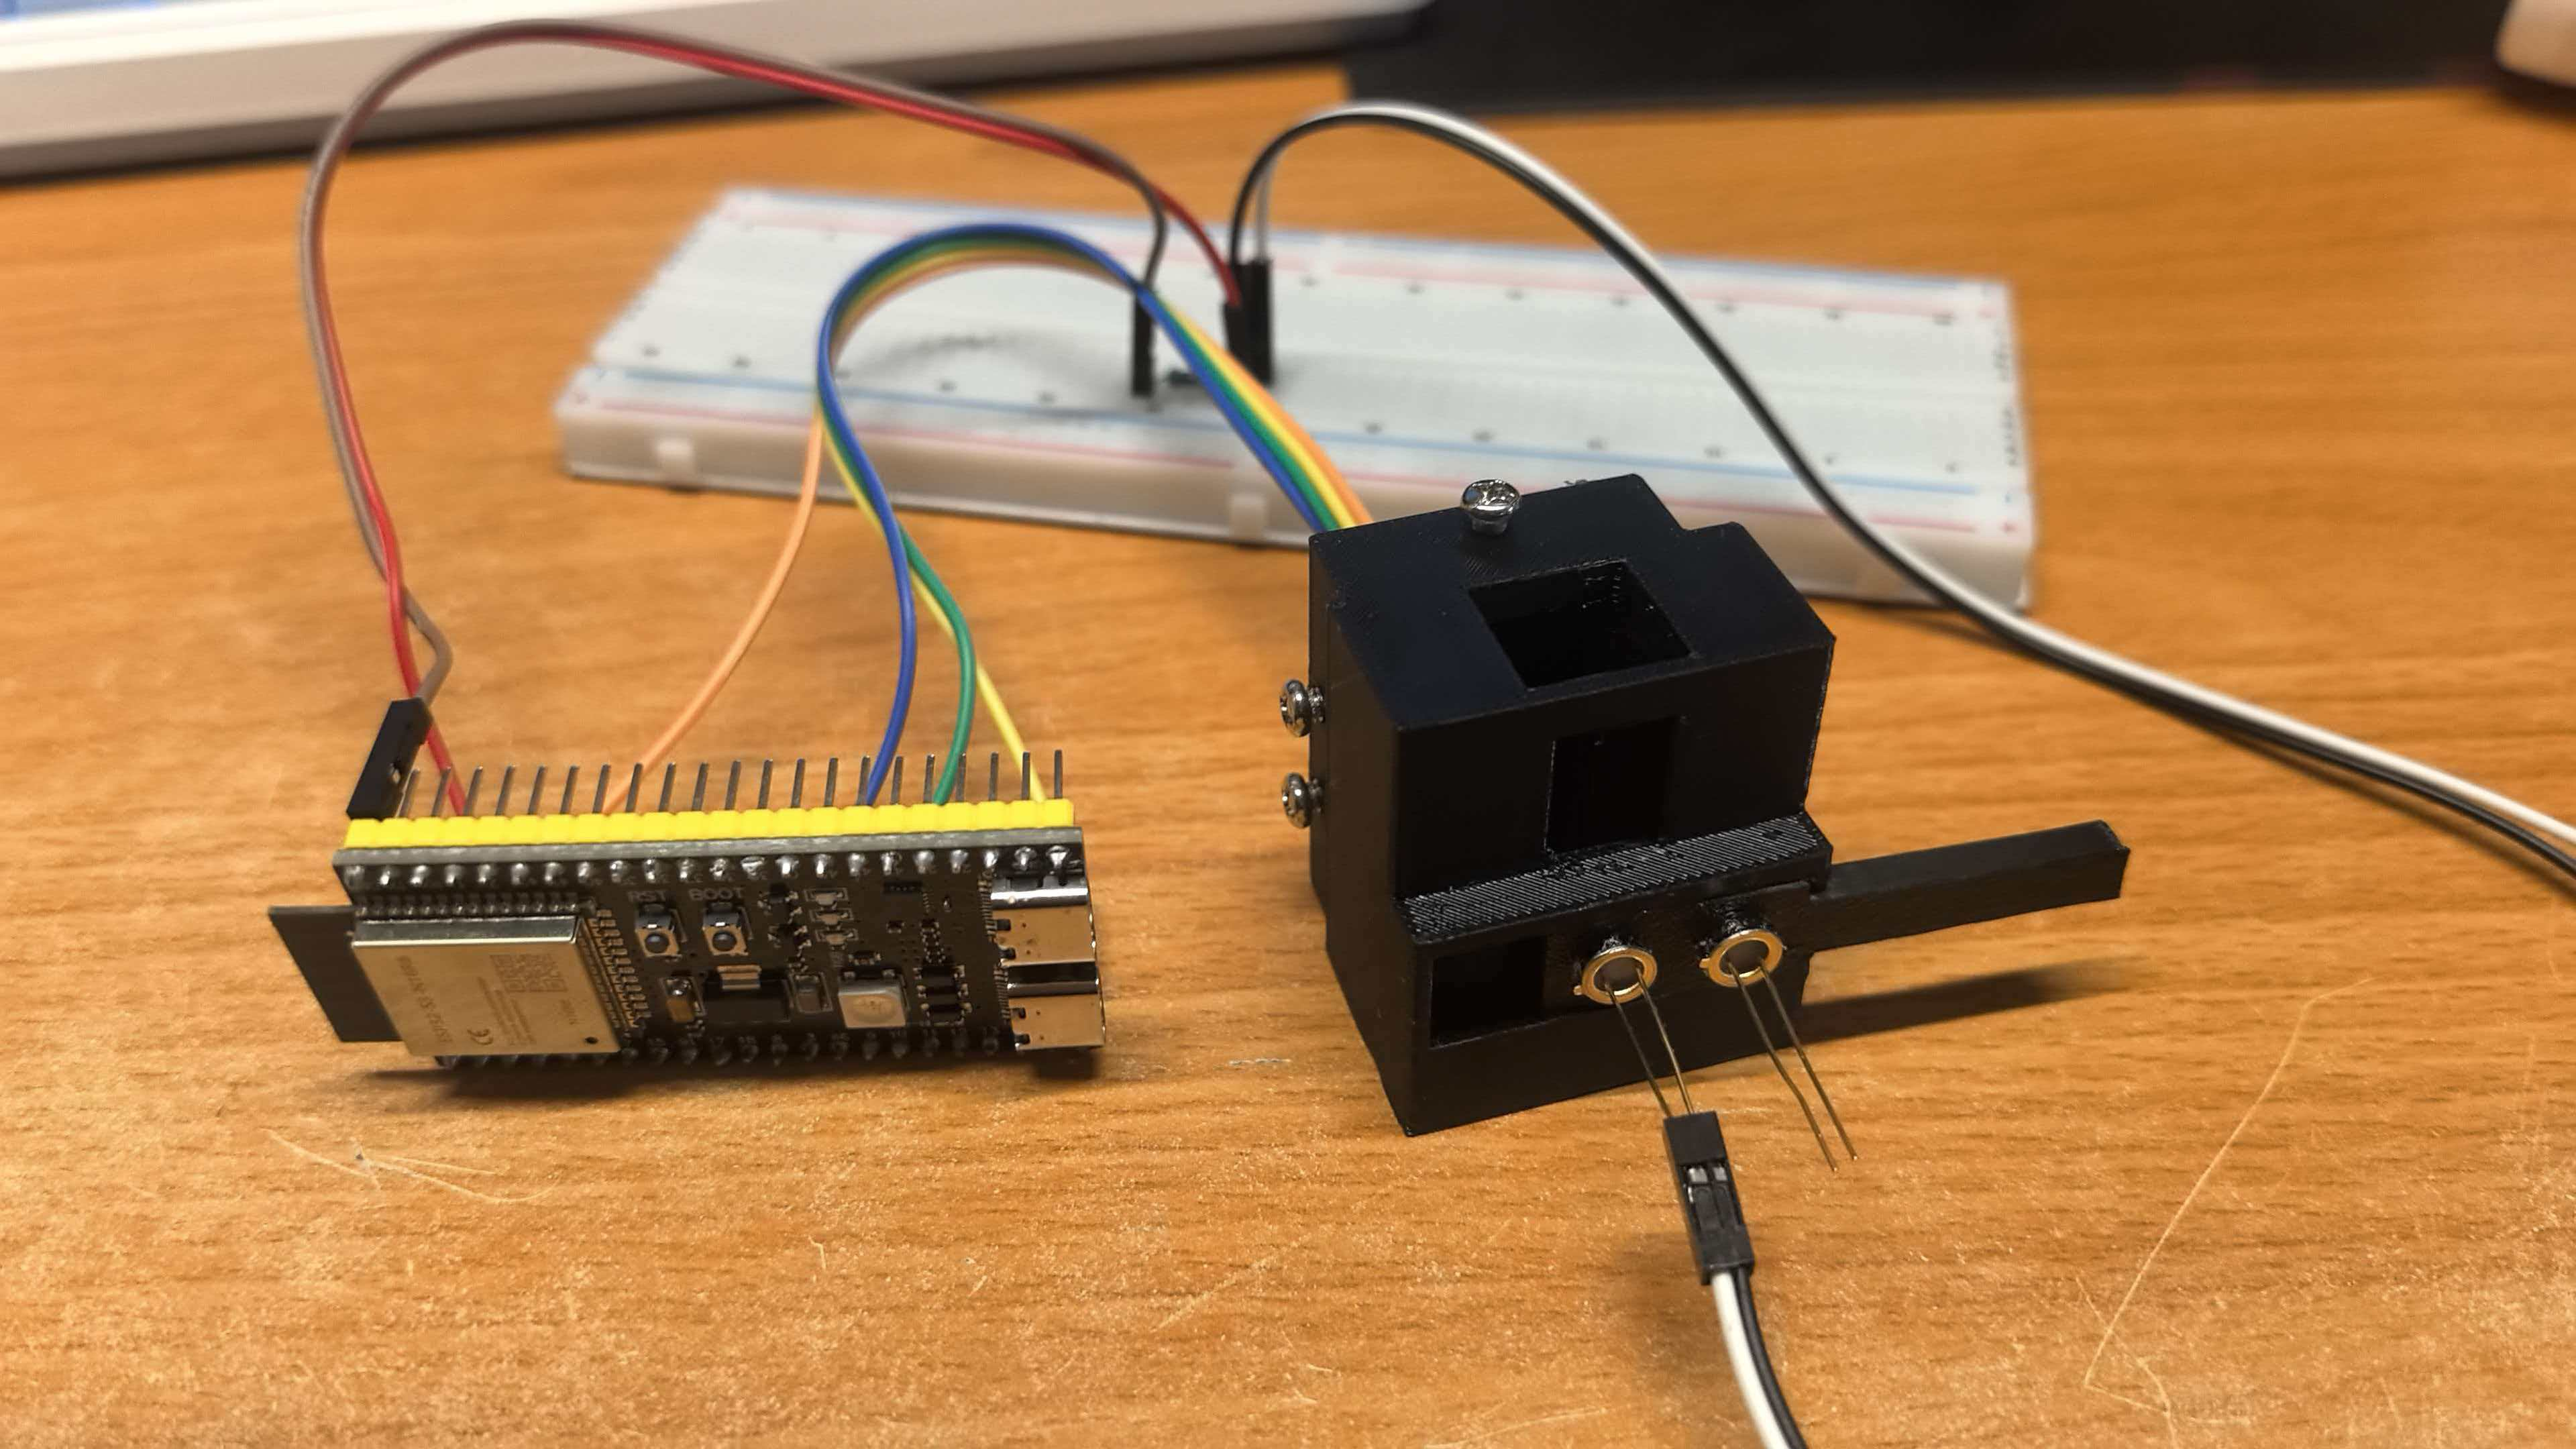
\includegraphics[width=0.7\textwidth]{../../hardware/figure/实物图.jpg}
\caption{检测装置实物 Demo 图}
\label{fig:hardware}
\end{figure}

\subsection{后续任务}

\begin{enumerate}
\item 完成 PCB 版本设计与焊接。
\item 实现离线缓存和断点续传。
\item 完成防水封装与连续运行测试。
\item 增加设备自检状态码。
\item 建立 72 小时连续运行稳定性测试。
\end{enumerate}

\subsection{验收标准}

\begin{enumerate}
\item 数据包完整率达到目标阈值。
\item 断网恢复后历史数据可补传。
\item 连续运行时长满足单轮任务需求。
\end{enumerate}

\section{无人机与投放装置}

\subsection{目标}

实现可重复、可校准、可追溯的投放流程。

\subsection{当前进度}

无人机尚未开发成功，当前仅完成部件采购与初步方案讨论。

\subsection{后续任务}

\begin{enumerate}
\item 第一步先完成无人机基础飞行成功标准定义（起飞、悬停、降落、返航）。
\item 完成空载试飞并记录至少 20 架次稳定日志。
\item 在空载稳定后再进行载荷试飞与返航安全策略验证。
\item 完成舵机或电磁投放机构联调，并建立投放偏差标定数据集。
\item 若第 2 步未达标，立即切换"人工布点 + 无人机模拟轨迹"备选流程，保证项目推进不断档。
\end{enumerate}

\subsection{验收标准}

\begin{enumerate}
\item 空载阶段：连续 20 架次无严重飞控异常。
\item 载荷阶段：悬停稳定性和返航逻辑通过测试。
\item 投放阶段：投放命中半径满足任务要求。
\item 安全阶段：故障触发时可自动中止并返航。
\end{enumerate}

%=============================================================================
\chapter{任务调度与系统中台}
%=============================================================================

\section{目标}

把模型结果自动转化为可执行任务，并实现全链路审计。

\section{输入}

\begin{enumerate}
\item 风险图与不确定性图。
\item 无人机状态和电量。
\item 天气窗口、禁飞区、人员值守信息。
\end{enumerate}

\section{输出}

\begin{enumerate}
\item 任务单与航点序列。
\item 投放时序和中止条件。
\item 单任务复盘报告。
\end{enumerate}

\section{验收标准}

\begin{enumerate}
\item 高峰时段任务生成可在可接受时间内完成。
\item 可行任务率与执行成功率满足阈值。
\item 每次任务都可回溯到模型版本和输入数据版本。
\item 在无人机未成功前，系统必须支持"模拟执行模式"，确保闭环算法可继续迭代。
\end{enumerate}

%=============================================================================
\chapter{Web 平台模块}
%=============================================================================

\section{目标}

构建服务团队与利益相关方的统一可视化平台。

\section{页面能力}

\begin{enumerate}
\item 实时地图：无人机轨迹、投放点、节点在线状态。
\item 风险看板：浓度预测热力图与分级预警。
\item 复盘页面：预测值与实测值偏差、任务成功率。
\item 告警中心：设备离线、异常漂移、极端风险提示。
\end{enumerate}

\section{当前状态}

当前为 Demo 页面，需优先完成以下两项最小化升级：
\begin{enumerate}
\item 接入真实或模拟实时数据流，不再仅展示静态样例。
\item 增加任务时间线与告警日志，支持评审追溯。
\end{enumerate}

当前网页 Demo 界面如下：

总览页示意：

\begin{figure}[htbp]
\centering
\includegraphics[width=0.85\textwidth]{../figure/网页总览图.webp}
\caption{水体藻毒素监测平台总览}
\label{fig:web-overview}
\end{figure}

设备配对与监控页示意：

\begin{figure}[htbp]
\centering
\includegraphics[width=0.85\textwidth]{../figure/设备配对图.webp}
\caption{采样设备连接与监控}
\label{fig:device-pair}
\end{figure}

数据分析页示意：

\begin{figure}[htbp]
\centering
\includegraphics[width=0.85\textwidth]{../figure/数据分析网页图.webp}
\caption{数据分析页面}
\label{fig:data-analysis}
\end{figure}

\section{验收标准}

\begin{enumerate}
\item 桌面端和移动端均可稳定访问。
\item 核心告警可在目标时延内推送。
\item 关键图表可导出用于答辩与报告。
\end{enumerate}

%=============================================================================
\chapter{模块间接口协议与数据流}
%=============================================================================

\section{系统数据流总览}

\begin{lstlisting}[language={},basicstyle=\small\ttfamily]
检测节点 (ESP32) --MQTT--> 数据中台 --HTTP--> Web 平台
                                |                      ^
                           数据库存储            模型推理 API
                                ^                      ^
                           历史数据 ----------> 预测模型
                                                     |
                                              风险预测结果
                                                     |
                                              任务调度引擎 --> 无人机/模拟执行
\end{lstlisting}

\section{接口定义}

\subsection{接口 A：检测节点 $\rightarrow$ 数据中台（上行数据）}

\begin{table}[htbp]
\centering
\caption{接口 A 参数}
\begin{tabular}{ll}
\toprule
\textbf{字段} & \textbf{说明} \\
\midrule
协议 & MQTT (QoS 1) \\
Topic & \texttt{sensor/\{device\_id\}/data} \\
频率 & 每 5 分钟上报一次 \\
数据格式 & JSON \\
\bottomrule
\end{tabular}
\end{table}

\begin{lstlisting}[language={},title={接口 A 数据示例}]
{
  "device_id": "ESP32-001",
  "timestamp": "2026-05-01T10:05:00Z",
  "battery_mv": 3700,
  "status": "NORMAL",
  "readings": {
    "water_temp": 22.5,
    "ph": 7.8,
    "turbidity": 15.3,
    "chla": 12.6,
    "dissolved_oxygen": 8.2
  }
}
\end{lstlisting}

\subsection{接口 B：预测模型 $\rightarrow$ 任务调度 / Web 平台}

\begin{table}[htbp]
\centering
\caption{接口 B 参数}
\begin{tabular}{ll}
\toprule
\textbf{字段} & \textbf{说明} \\
\midrule
协议 & HTTP REST API \\
路径 & \texttt{POST /api/v1/predict} \\
数据格式 & JSON \\
\bottomrule
\end{tabular}
\end{table}

\begin{lstlisting}[language={},title={接口 B 数据示例}]
{
  "region": "lake_erie",
  "forecast_hours": 48,
  "input_features": { "...": "..." },
  "output": {
    "risk_level": "HIGH",
    "probability": 0.87,
    "predicted_concentration_ugl": 3.2,
    "confidence_lower": 1.8,
    "confidence_upper": 5.6,
    "model_version": "ensemble_v2.1"
  }
}
\end{lstlisting}

\subsection{接口 C：任务调度 $\rightarrow$ 无人机 / 模拟执行器}

\begin{table}[htbp]
\centering
\caption{接口 C 参数}
\begin{tabular}{ll}
\toprule
\textbf{字段} & \textbf{说明} \\
\midrule
协议 & HTTP REST API \\
路径 & \texttt{POST /api/v1/task} \\
数据格式 & JSON \\
\bottomrule
\end{tabular}
\end{table}

\begin{lstlisting}[language={},title={接口 C 数据示例}]
{
  "task_id": "TASK-20260501-001",
  "mode": "SIMULATED",
  "waypoints": [
    {"lat": 41.73, "lng": -83.04, "alt_m": 30, "action": "HOVER"},
    {"lat": 41.74, "lng": -83.05, "alt_m": 15, "action": "DROP"}
  ],
  "drop_count": 3,
  "abort_conditions": {
    "battery_pct_below": 20,
    "wind_speed_ms_above": 8.0
  },
  "model_version": "ensemble_v2.1",
  "input_data_hash": "sha256:abc123"
}
\end{lstlisting}

\subsection{接口 D：数据中台 $\rightarrow$ Web 平台（WebSocket 推送）}

\begin{table}[htbp]
\centering
\caption{接口 D 参数}
\begin{tabular}{ll}
\toprule
\textbf{字段} & \textbf{说明} \\
\midrule
协议 & WebSocket \\
事件类型 & \texttt{sensor\_update} / \texttt{risk\_alert} / \texttt{task\_status} \\
\bottomrule
\end{tabular}
\end{table}

\begin{lstlisting}[language={},title={接口 D 数据示例}]
{
  "event": "risk_alert",
  "timestamp": "2026-05-01T10:10:00Z",
  "region": "lake_erie",
  "risk_level": "HIGH",
  "message": "MIC 检出概率 87%，预测浓度 3.2 ug/L"
}
\end{lstlisting}

\section{设备状态码定义}

\begin{table}[htbp]
\centering
\caption{设备状态码}
\begin{tabular}{lll}
\toprule
\textbf{状态码} & \textbf{含义} & \textbf{处理建议} \\
\midrule
\texttt{NORMAL} & 正常运行 & 无需操作 \\
\texttt{LOW\_BATTERY} & 电量低于 20\% & 安排回收更换 \\
\texttt{SENSOR\_WARN} & 传感器读数异常 & 检查探头，触发定标 \\
\texttt{OFFLINE} & 设备离线超 15 分钟 & 排查网络或硬件 \\
\texttt{WATER\_INGRESS} & 检测到湿度异常 & 安排回收检查封装 \\
\bottomrule
\end{tabular}
\end{table}

%=============================================================================
\chapter{12 周执行排期（2026-04-21 $\sim$ 2026-07-13）}
%=============================================================================

\begin{quote}
注：模型模块已完成全流程（第 1--2 周的模型任务已提前完成），排期据此调整。
\end{quote}

\begin{longtable}{cl p{6cm} p{4cm}}
\toprule
\textbf{周次} & \textbf{日期} & \textbf{主要任务} & \textbf{交付物} \\
\midrule
\endfirsthead
\toprule
\textbf{周次} & \textbf{日期} & \textbf{主要任务} & \textbf{交付物} \\
\midrule
\endhead
\bottomrule
\endlastfoot
第 1 周 & 04/21--04/27 & 冻结 Demo 版本，统一数据字典和接口协议，模型上线推理 API & 接口协议文档、推理 API \\
第 2 周 & 04/28--05/04 & 模型训练流程 \textcolor{green!60!black}{\textbf{已完成}} $\rightarrow$ 补充预测区间输出和在线推理联调 & 在线推理服务、不确定性量化 \\
第 3 周 & 05/05--05/11 & 网页 Demo 接入实时流，打通任务时间线与告警日志 & 实时数据流、告警推送 \\
第 4 周 & 05/12--05/18 & ESP32 进入 PCB 设计评审，完成通信与缓存联调 & PCB 设计图、缓存测试报告 \\
第 5 周 & 05/19--05/25 & 无人机基础飞行调试：起飞、悬停、降落、返航 & 飞行日志、问题清单 \\
第 6 周 & 05/26--06/01 & 空载 20 架次稳定性测试；若未达标则启动人工布点备选 & 稳定性报告或备选流程文档 \\
第 7 周 & 06/02--06/08 & 任务调度最小版本：支持真实执行与模拟执行双模式 & 调度引擎 v0.1 \\
第 8 周 & 06/09--06/15 & 投放机构台架联调，输出投放偏差标定方案 & 投放偏差数据集 \\
第 9 周 & 06/16--06/22 & 首次半闭环演练（模型+调度+网页+模拟/真实执行） & 演练复盘报告 \\
第 10 周 & 06/23--06/29 & 修复半闭环瓶颈，推进自动训练与版本回滚 & 修复清单、自动化流水线 \\
第 11 周 & 06/30--07/06 & 外场最小闭环演练并形成失败复盘 & 外场报告、证据包 \\
第 12 周 & 07/07--07/13 & 固化答辩证据包、对照实验结果与演示脚本 & 答辩完整资料 \\
\end{longtable}

%=============================================================================
\chapter{风险清单与备选方案}
%=============================================================================

\begin{enumerate}
\item 传感器漂移：触发信号为短时波动异常，缓解为定标与温补，兜底为邻近节点投票。
\item 网络不稳定：触发为丢包与延迟升高，缓解为本地队列，兜底为任务后集中回传。
\item 投放偏差过大：触发为命中率下降，缓解为风偏修正，兜底为近岸人工布设。
\item 续航不足：触发为任务中低电量，缓解为调度约束，兜底为分段任务。
\item 新水域泛化差：触发为误差抬升，缓解为迁移学习，兜底为规则阈值预警。
\item 标签延迟：触发为补标堆积，缓解为弱监督流程，兜底为冻结模型版本。
\item 防水失效：触发为湿度告警，缓解为浸泡测试，兜底为双层封装。
\item 调度超时：触发为任务生成延迟，缓解为启发式先求可行解，兜底为模板航线。
\item 禁飞限制：触发为审批失败，缓解为提前备案，兜底为岸基采样验证。
\item 公众疑虑：触发为负面反馈上升，缓解为透明沟通，兜底为先展示非活体流程。
\item 接口不一致：触发为联调频繁失败，缓解为接口契约，兜底为适配层转换。
\item 演示故障：触发为彩排不稳定，缓解为故障注入演练，兜底为离线回放方案。
\end{enumerate}

%=============================================================================
\chapter{iGEM 评审对齐策略}
%=============================================================================

\begin{enumerate}
\item \textbf{Innovation}：强调预测-投放-反馈-再学习的闭环创新，而非单一预测模型。
\item \textbf{Engineering}：保留每轮设计、构建、测试、学习证据链，体现工程迭代。
\item \textbf{Human Practices}：引入环保部门、社区、渔业用户反馈并反哺技术决策。
\item \textbf{Safety}：同步覆盖生物安全与飞行安全，设置可执行中止和回滚机制。
\item \textbf{Integrated Human Practices}：把访谈结果映射为阈值、任务规则和界面信息层级。
\item \textbf{Presentation}：用一张总闭环图和一条真实任务时间线讲清系统价值。
\end{enumerate}

%=============================================================================
\chapter{本周立即执行清单}
%=============================================================================

\begin{enumerate}
\item 输出一页当前状态基线表，明确哪些是 Demo、哪些已可联调。
\item 冻结模型 Demo 输入输出字段，新增风险分级与不确定性字段。
\item 冻结网页 Demo 页面结构，优先接入实时流与告警日志。
\item 完成 ESP32 断网补传测试并记录失败场景。
\item 给无人机制定"成功标准四件套"：起飞、悬停、降落、返航。
\item 完成无人机首轮空载调试并输出问题清单。
\item 制定无人机未成功时的人工布点备选流程。
\item 输出任务调度模拟执行模式的最小接口定义。
\item 召开一次闭环联调会，逐段确认阻塞点和负责人。
\item 形成本周复盘文档，给出下周只做三件最关键事情。
\end{enumerate}

\end{document}
